%To compile as handout, use
%pdflatex "\def\ishandout{1} \input{filename.tex}"
%Defaults to non-handout mode (with slide reveals)
\ifdefined\ishandout
  \documentclass[handout]{beamer}
\else
  \documentclass{beamer}
\fi
 
\usepackage{econ103slides} 

\date{Lecture \# 13}
\begin{document} 

%%%%%%%%%%%%%%%%%%%%%%%%%%%%%%%%%%%%%%%%

\begin{frame}[plain]
	\titlepage 
	

\end{frame} 

%%%%%%%%%%%%%%%%%%%%%%%%%%%%%%%%%%%%%%%%
\begin{frame}
\Huge \begin{center}
Continuous RVs -- Part III
\end{center}
\end{frame}
%%%%%%%%%%%%%%%%%%%%%%%%%%%%%%%%%%%%%%%%
\begin{frame}
\begin{figure}
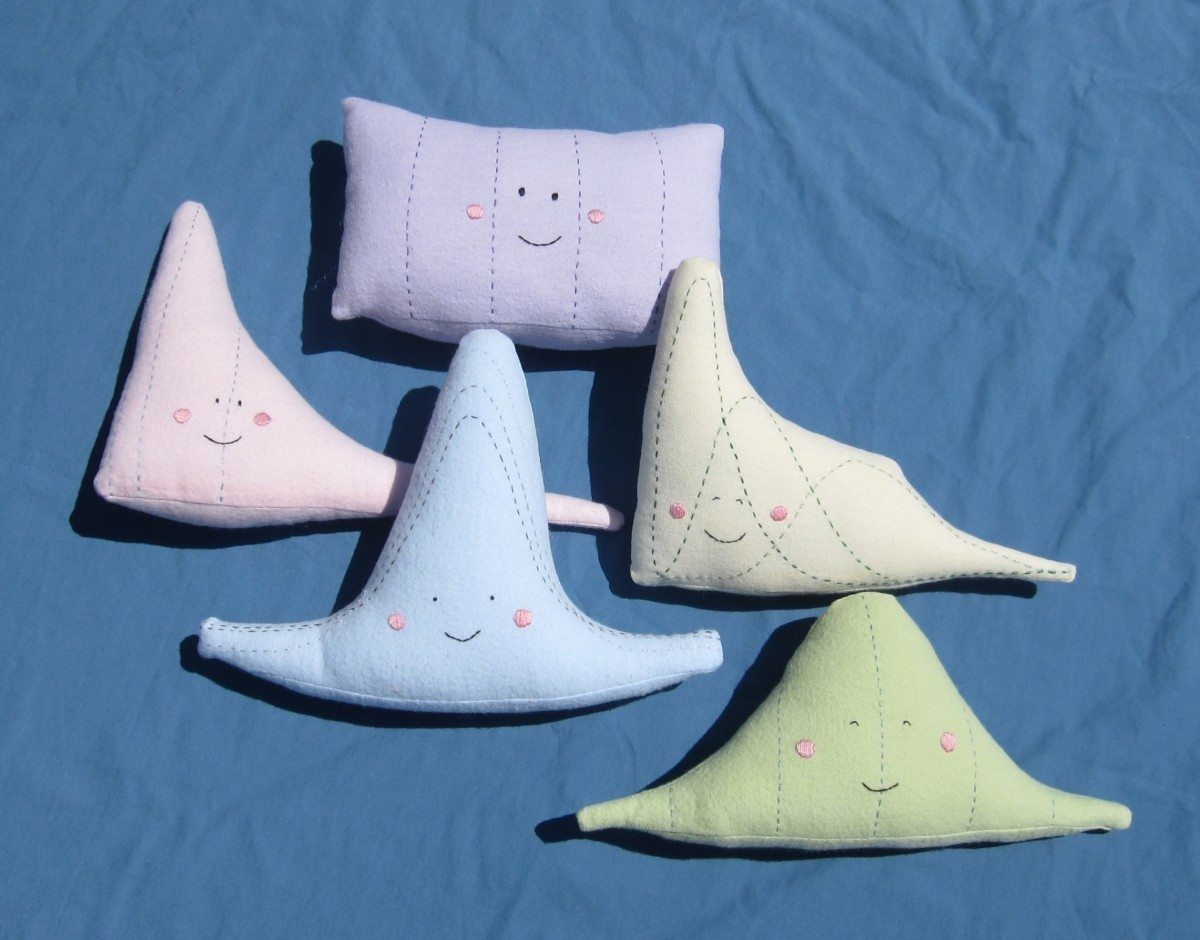
\includegraphics[scale = 0.2]{./images/normal_friends}
\caption{The Normal Distribution and Friends.}
\end{figure}
\end{frame}
%%%%%%%%%%%%%%%%%%%%%%%%%%%%%%%%%%%%%%%%
\begin{frame}
	\frametitle{\normalsize \href{http://ditraglia.com/Econ103Public/Rtutorials/friends_of_normal.html}{http://ditraglia.com/Econ103Public/Rtutorials/friends\_of\_normal.html}}
\framesubtitle{Source Code on my \href{https://github.com/fditraglia/Econ103Public/blob/master/Rtutorials/friends_of_normal.R}{\fbox{Github Page}}}



\begin{figure}
	\fbox{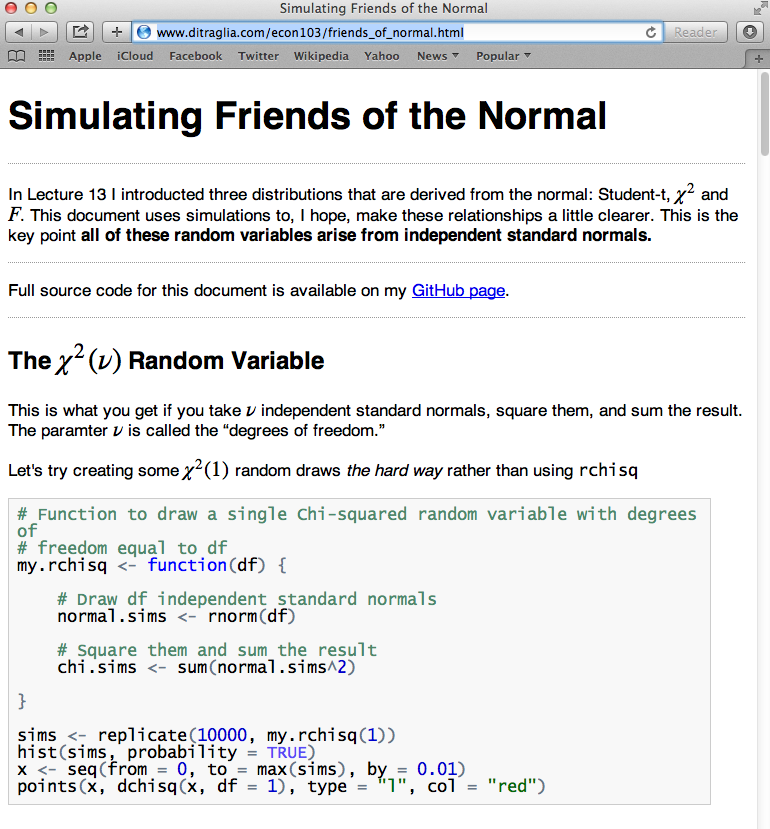
\includegraphics[scale = 0.2]{./images/normal_friends_screenshot}}
\end{figure}

\end{frame}

%%%%%%%%%%%%%%%%%%%%%%%%%%%%%%%%%%%%%%%%

\begin{frame}
\frametitle{Functions of Independent RVs are Independent}

If $X$ and $Y$ are independent random variables and $g$ and $h$ are functions, then the random variables $g(X)$ and $h(Y)$ are also independent.

\end{frame}



%%%%%%%%%%%%%%%%%%%%%%%%%%%%%%%%%%%%%%%%
\begin{frame}
\begin{figure}
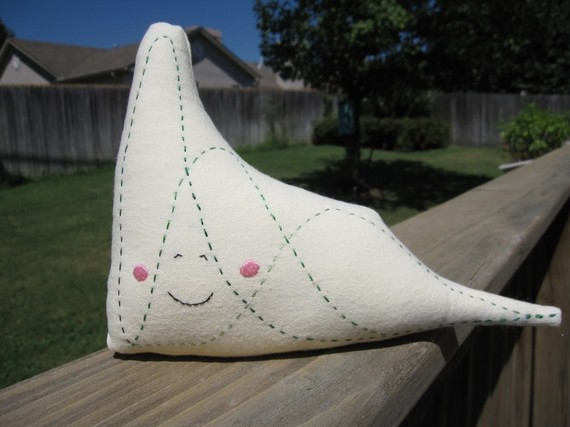
\includegraphics[scale = 0.45]{./images/chisq_etsy1}
\caption{PDF for $\chi^2$-Distribution}
\end{figure}
\end{frame}

%%%%%%%%%%%%%%%%%%%%%%%%%%%%%%%%%%%%%%%%
\begin{frame}
\begin{figure}
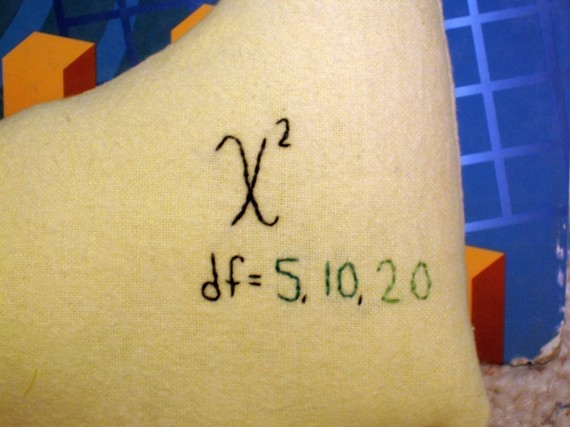
\includegraphics[scale = 0.45]{./images/chisq_etsy2}
\end{figure}
\end{frame}
%%%%%%%%%%%%%%%%%%%%%%%%%%%%%%%%%%%%%%%%
\begin{frame}
\frametitle{$\chi^2$ Random Variable}
Let $X_1, \hdots, X_\nu \sim \mbox{iid } N(0,1)$. Then,
	$$\left(X_1^2 + \hdots + X_\nu^2  \right)\sim \chi^2(\nu)$$
	where the parameter $\nu$ is the \emph{degrees of freedom}
	
	\vspace{1em}
	\pause
	\alert{Support = $(0, \infty)$}\\
	\vspace{1em}
\end{frame}




%%%%%%%%%%%%%%%%%%%%%%%%%%%%%%%%%%%%%%%%

\begin{frame}
\frametitle{$\chi^2$ PDFs}

\begin{figure}
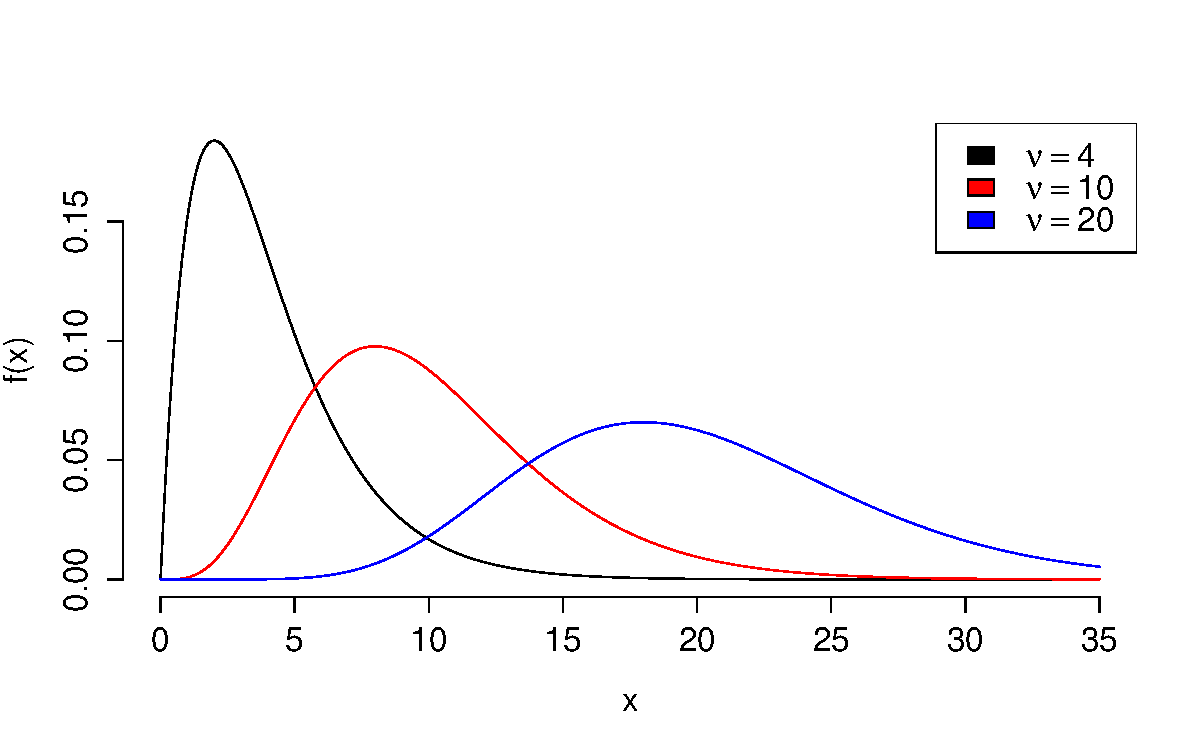
\includegraphics[scale = 0.58]{./images/chisq}
\end{figure}
\end{frame}

%%%%%%%%%%%%%%%%%%%%%%%%%%%%%%%%%%%%%%%%
%\begin{frame}
%\begin{figure}
%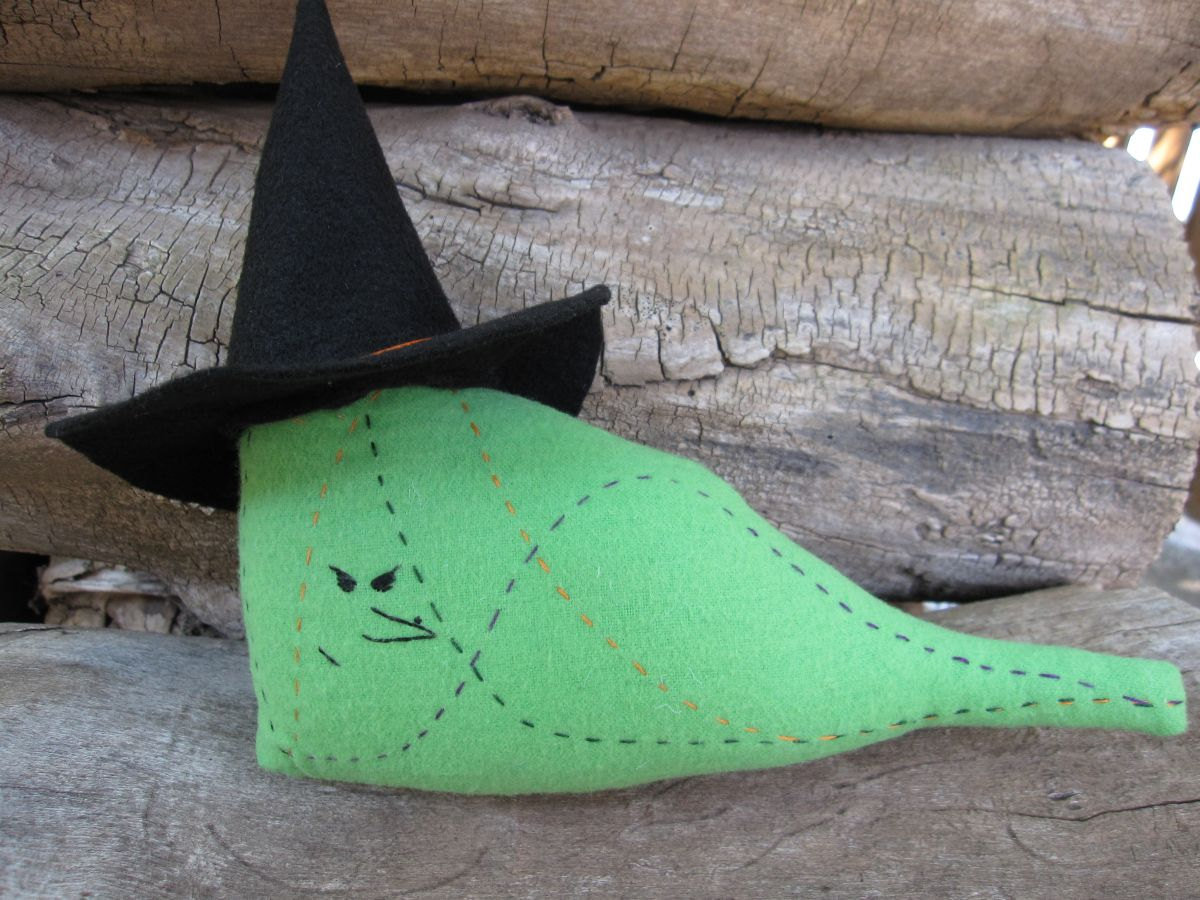
\includegraphics[scale = 0.45]{./images/chisq_etsy_witch}
%\caption{$\chi^2$ PDF -- Halloween Edition}
%\end{figure}
%\end{frame}
%%%%%%%%%%%%%%%%%%%%%%%%%%%%%%%%%%%%%%%%

\begin{frame}
\begin{figure}
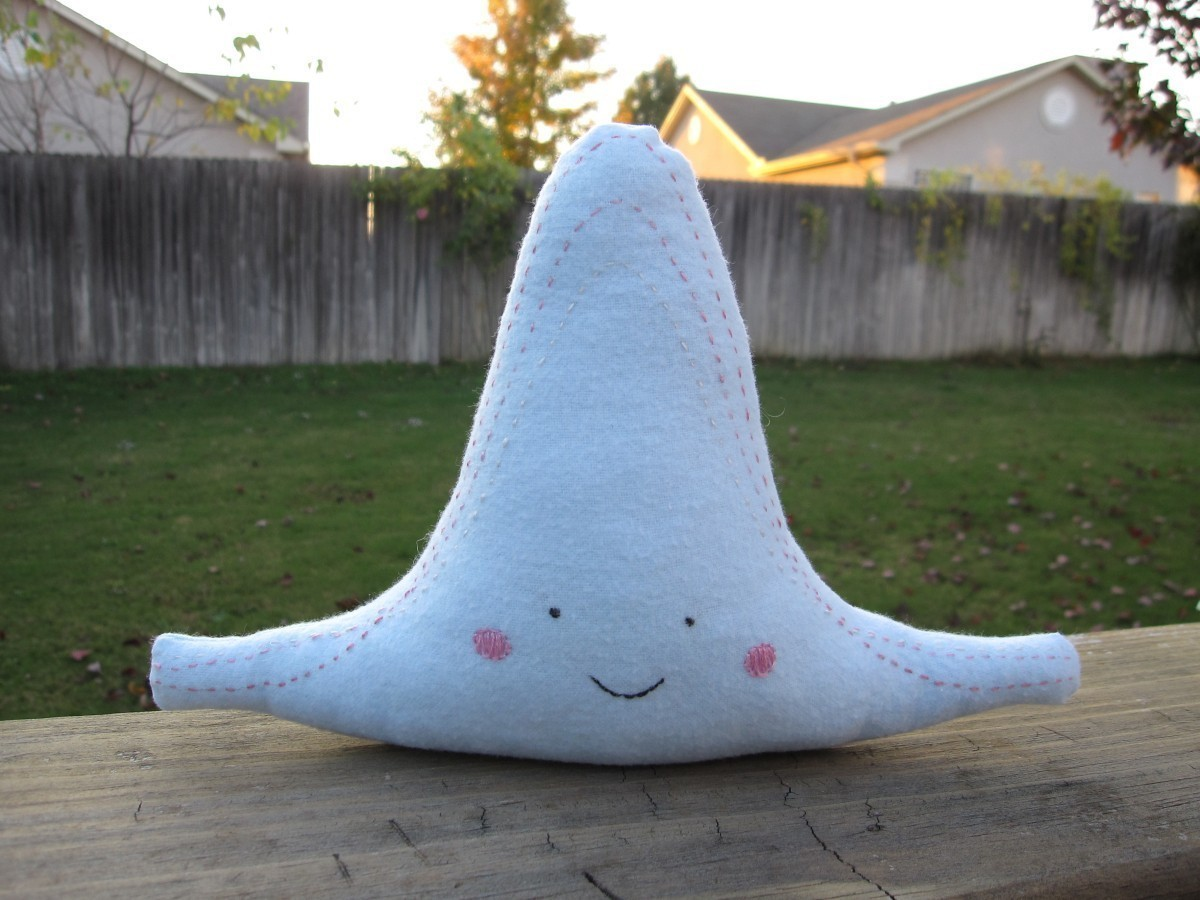
\includegraphics[scale = 0.2]{./images/t_etsy1}
\caption{PDF for Student-t Distribution}
\end{figure}
\end{frame}

%%%%%%%%%%%%%%%%%%%%%%%%%%%%%%%%%%%%%%%%
\begin{frame}
\begin{figure}
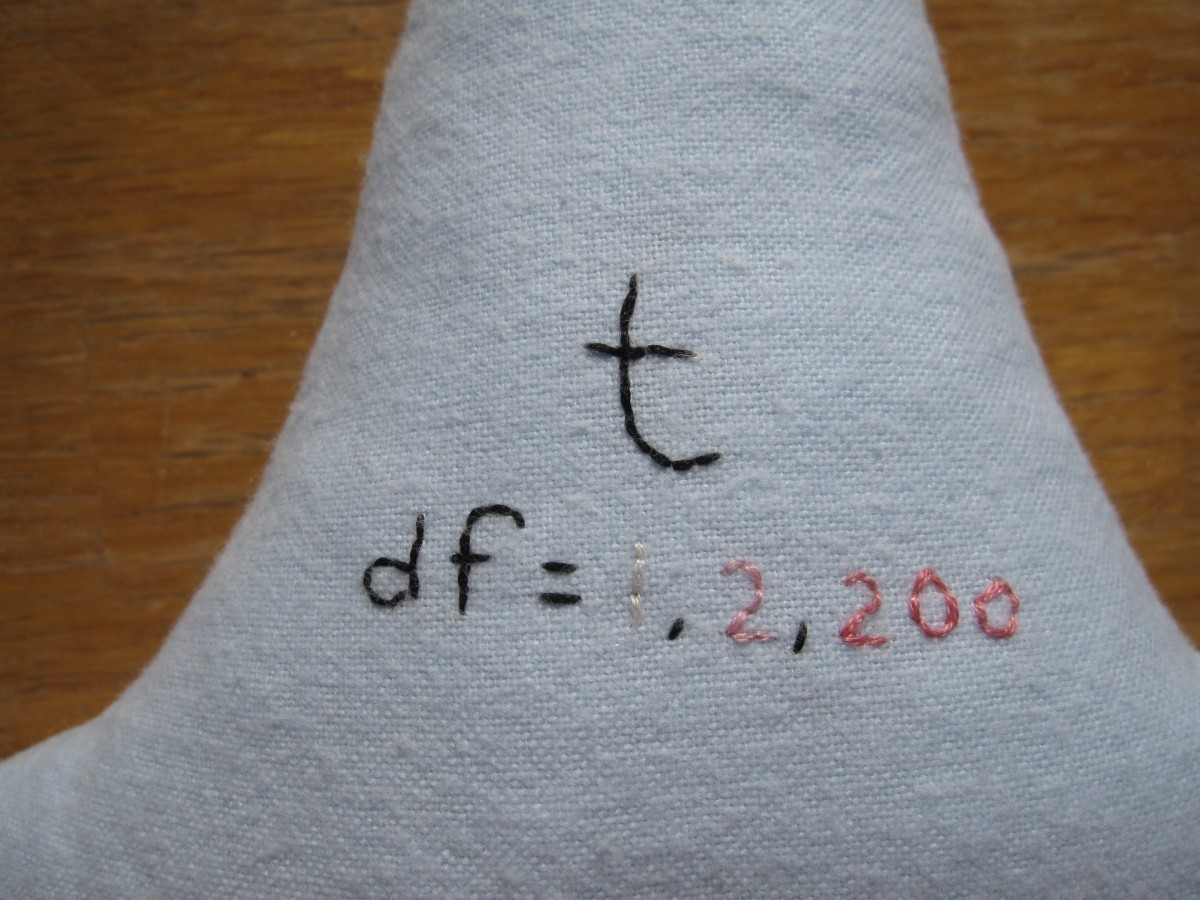
\includegraphics[scale = 0.2]{./images/t_etsy2}
\end{figure}
\end{frame}

%%%%%%%%%%%%%%%%%%%%%%%%%%%%%%%%%%%%%%%%

\begin{frame}
\frametitle{Student-t Random Variable}
Let $X \sim N(0,1)$ independent of $Y \sim \chi^2(\nu)$. Then,
$$\frac{X}{\sqrt{Y/\nu}}\sim t(\nu)$$
where the parameter $\nu$ is the degrees of freedom.

\pause

\begin{itemize}
	\item Support = $(-\infty, \infty)$
	\item As $\nu \rightarrow \infty$, $t \rightarrow$ Standard Normal.
	\item Symmetric around zero, but mean and variance may not exist!
	\item Degrees of freedom $\nu$ control ``thickness of tails''
\end{itemize}
\vspace{1em}


\end{frame}

%%%%%%%%%%%%%%%%%%%%%%%%%%%%%%%%%%%%%%%%
\begin{frame}
\frametitle{Student-t PDFs}

\begin{figure}
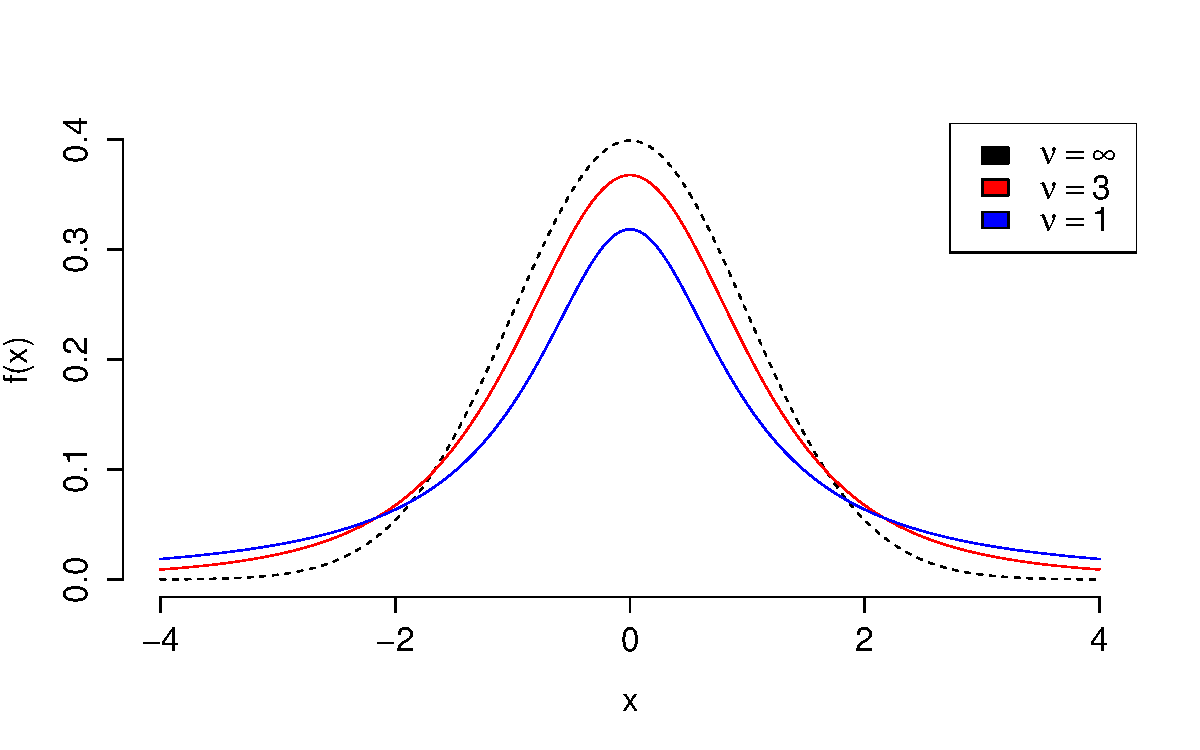
\includegraphics[scale = 0.58]{./images/tpdf}
\end{figure}
\end{frame}

%%%%%%%%%%%%%%%%%%%%%%%%%%%%%%%%%%%%%%%%
\begin{frame}
\frametitle{F Random Variable}
Suppose $X \sim \chi^2(\nu)$ independent of $Y \sim \chi^2(\omega)$. Then,
	$$\frac{X/\nu}{Y/\omega} \sim F(\nu, \omega)$$
where $\nu$ is the numerator degrees of freedom and $\omega$ is the denominator degrees of freedom.
\vspace{1em}


\alert{Support = $(0, \infty)$}\\

\end{frame}




%%%%%%%%%%%%%%%%%%%%%%%%%%%%%%%%%%%%%%%%
\begin{frame}
\frametitle{F PDFs}

\begin{figure}
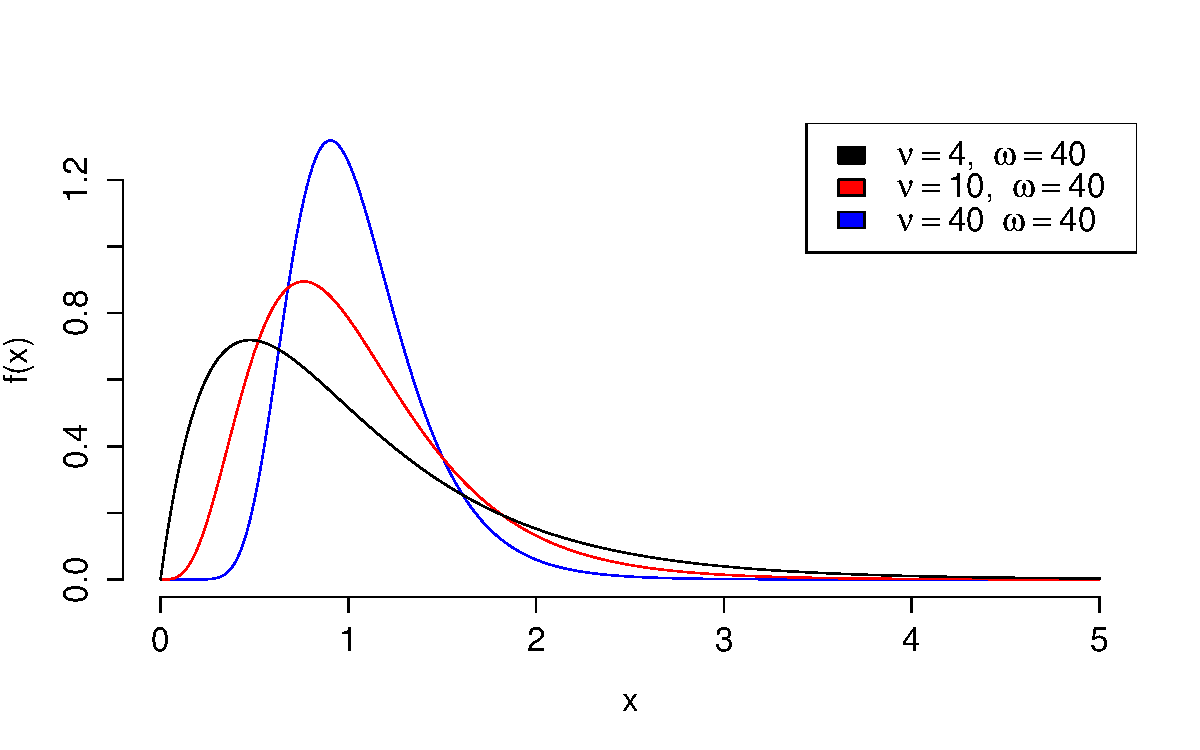
\includegraphics[scale = 0.58]{./images/Fdist}
\end{figure}
\end{frame}

%%%%%%%%%%%%%%%%%%%%%%%%%%%%%%%%%%%%%%%%

\begin{frame}
\frametitle{R Commands -- CDFs and Quantile Functions}
$F(x) = P(X\leq x)$ is the CDF, $Q(p) = F^{-1}(p)$ the Quantile Function
\footnotesize
\begin{table}
\begin{tabular}{l|ll}
&$F(x)$&$Q(p)$\\
\hline
$N(\mu,\sigma^2)$ &\texttt{pnorm(x, mean = $\mu$,  sd = $\sigma$)}&\texttt{qnorm(p, mean = $\mu$,  sd = $\sigma$)}\\
$\chi^2(\nu)$&\texttt{pchisq(x, df = $\nu$)}&\texttt{qchisq(p, df = $\nu$)}\\
$t(\nu)$&\texttt{pt(x, df = $\nu$)}&\texttt{qt(p, df = $\nu$)}\\
$F(\nu,\omega)$&\texttt{pf(x, df1 = $\nu$, df2 = $\omega$)}&\texttt{qf(p, df1 = $\nu$, df2 = $\omega$)}
\end{tabular}
\end{table}
\vspace{1em}
\normalsize
\alert{Mnemonic: ``p'' is for Probability, ``q'' is for Quantile.}

\end{frame}
%%%%%%%%%%%%%%%%%%%%%%%%%%%%%%%%%%%%%%%%
\begin{frame}
\frametitle{R Commands -- PDFs and Random Draws}
\footnotesize
\begin{table}
\begin{tabular}{l|ll}
&$f(x)$&Make \texttt{n} iid Random Draws\\
\hline
$N(\mu,\sigma^2)$ &\texttt{dnorm(x, mean = $\mu$,  sd = $\sigma$)}&\texttt{rnorm(n, mean = $\mu$,  sd = $\sigma$)}\\
$\chi^2(\nu)$&\texttt{dchisq(x, df = $\nu$)}&\texttt{rchisq(n, df = $\nu$)}\\
$t(\nu)$&\texttt{dt(x, df = $\nu$)}&\texttt{rt(n, df = $\nu$)}\\
$F(\nu,\omega)$&\texttt{df(x, df1 = $\nu$, df2 = $\omega$)}&\texttt{rf(n, df1 = $\nu$, df2 = $\omega$)}
\end{tabular}
\end{table}
\vspace{1em}
\normalsize
\alert{Mnemonic: ``d'' is for Density, ``r'' is for Random.}

\end{frame}
%%%%%%%%%%%%%%%%%%%%%%%%%%%%%%%%%%%%%%%%


\begin{frame}
\frametitle{Example: $X_1, X_2, X_3 \sim \mbox{iid } N(0, 1)$}
\begin{block}{What is the distribution of $Y_1 = X_1^2 + X_2^2$?}\pause
Sum of squares of two indep.\ std.\ normals $\Rightarrow \alert{Y_1 \sim \chi^2(2)}$
\end{block}
\pause
\begin{block}{What is the distribution of $Y_2 = (Y_1/2)/(X_3^2)$?}
\pause
$Y_1 \sim \chi^2(2)$ and $X_3^2 \sim \chi^2(1)$\\
\pause
\vspace{1em}
Hence $Y_2 =$ ratio of two indep.\ $\chi^2$ RVs, each divided by its degrees of freedom $\Rightarrow \alert{Y_2 \sim F(2,1)}$
\end{block}
\pause
\begin{block}{What is the distribution of $Z = X_3/\sqrt{Y_1/2}$?}
\pause
Ratio of standard normal and square root of independent $\chi^2$ RV divided by its degrees of freedom $\Rightarrow \alert{Z \sim t(2)}$
\end{block}
\end{frame}
%%%%%%%%%%%%%%%%%%%%%%%%%%%%%%%%%%%%%%%%
\begin{frame}
\frametitle{Suppose $X_1, X_2, \sim \mbox{iid } N(\mu, \sigma^2)$ \hfill 
\includegraphics[scale = 0.05]{./images/clicker}}
Let $Y = \left( X_1 - \mu\right)^2 + \left( X_2 - \mu\right)^2$. What is the distribution of $Y/\sigma^2$?

\begin{enumerate}[(a)]
	\item $F(2,1)$
	\item $\chi^2(2)$
	\item $t(2)$
	\item $N(\mu, \sigma)$
	\item None of the above
\end{enumerate}

\end{frame}
%%%%%%%%%%%%%%%%%%%%%%%%%%%%%%%%%%%%%%%%
\begin{frame}
\frametitle{$Y_1 \sim \chi^2(2),\;\;\;\; Y_2 \sim F(2,1),\;\;\;\; Z \sim t(2)$}
\begin{block}{What is the median of $Y_1$?}
\pause
\texttt{qchisq(0.5, df = 2)}$\approx 1.4$
\end{block}
\pause
\begin{block}{What is $P(Y_2 \leq 5)$?}
\pause
\texttt{pf(5, df1 = 2, df2 = 1)}$\approx 0.7$
\end{block}
\pause
\begin{block}{What value of $c$ gives $P(-c\leq Z \leq c) = 0.5$?}
Use Symmetry (like normal) \\
$c=$\texttt{qt(0.75, df = 2)}$\approx 0.8$ 
\pause
\\or equivalently $-c =$\texttt{qt(0.25, df = 2)}$\approx -0.8$
\end{block}

\end{frame}
%%%%%%%%%%%%%%%%%%%%%%%%%%%%%%%%%%%%%%%%

\end{document}
